\documentclass[journal]{IEEEtran}
\usepackage{amsmath,amssymb,amsfonts}
\usepackage{graphicx}
\usepackage{booktabs}
\usepackage{siunitx}
\usepackage{xcolor}
\usepackage{url}
\usepackage{balance}
\usepackage[hidelinks]{hyperref}
\hypersetup{
  pdftitle={Complementary-Filtered Residual World Models for Receding-Horizon Control of Nonlinear Systems},
  pdfauthor={},pdfsubject={},pdfkeywords={}
}
\newcommand{\method}{CFR-WM}
\newcommand{\vect}[1]{\mathbf{#1}}
% Generated only from locked results/confirmatory_analysis artifacts.
\newcommand{\PrimaryBaseline}{PGNN-style}
\newcommand{\PrimaryDifference}{-0.0098}
\newcommand{\PrimaryCILow}{-0.0121}
\newcommand{\PrimaryCIHigh}{-0.0075}
\newcommand{\PrimaryImprovement}{8.97}
\newcommand{\PrimaryRelativeCILow}{6.88}
\newcommand{\PrimaryRelativeCIHigh}{10.95}
\newcommand{\PrimaryPValue}{0.00391}
\newcommand{\PrimaryDecision}{supported}
\newcommand{\PrimaryInterpretation}{supports the prespecified practical-gain claim}
\newcommand{\RobustnessDecision}{not supported}
\newcommand{\RobustnessInterpretation}{does not support the gated robustness claim}
\newcommand{\CorruptImprovement}{12.05}
\newcommand{\CorruptRelativeCILow}{10.51}
\newcommand{\CorruptRelativeCIHigh}{13.49}
\newcommand{\CorruptPValue}{0.00391}
\newcommand{\CleanImprovement}{-13.08}
\newcommand{\CleanRelativeCILow}{-20.60}
\newcommand{\CleanRelativeCIHigh}{-5.67}
\newcommand{\CleanPValue}{0.95703}
\newcommand{\CFRNRMSE}{0.0998}
\newcommand{\PGNNNRMSE}{0.1096}
\newcommand{\BestMethod}{CFR-WM}
\newcommand{\BestNRMSE}{0.0998}
\newcommand{\BestGain}{0.50}
\newcommand{\OneStepImprovement}{59.38}
\newcommand{\OneStepRelativeCILow}{48.88}
\newcommand{\OneStepRelativeCIHigh}{68.88}
\newcommand{\OneStepHolmP}{0.03906}
\newcommand{\CellsWorseTen}{3}
\newcommand{\CartpoleCleanChange}{+47.3}
\newcommand{\VanDerPolCleanChange}{+19.4}
\newcommand{\DuffingCleanChange}{+24.4}
\newcommand{\IDCorruptFavoredCount}{5}
\newcommand{\IDCorruptCellCount}{5}
\newcommand{\IDCorruptLeastChange}{-13.3}
\newcommand{\IDCorruptMostChange}{-34.8}
\newcommand{\AllMetricsFinite}{yes}
\newcommand{\UniqueDataHashes}{40}
\newcommand{\ConfirmatoryRuns}{440}
\newcommand{\ConfirmatoryTrajectories}{126{,}720}

\newcommand{\PosthocBestResidualScale}{0}
\newcommand{\ProjectionMissingEntries}{5404}
\newcommand{\ProjectionChangedFraction}{75.4}
\newcommand{\ProjectionMeanChange}{0.0328}
\newcommand{\ProjectionPChange}{0.1374}
\newcommand{\ProjectionMaxChange}{0.3848}
\newcommand{\CFRLatencyMean}{0.416}
\newcommand{\CFRLatencySD}{0.015}
\newcommand{\ResidualReconstructionDifference}{0.00e+00}
\newcommand{\ExternalMeanReconstructionDifference}{0.00e+00}

% Generated from verified saved external forecasts.
\newcommand{\ExternalTestFlights}{3}
\newcommand{\ExternalFinalSeeds}{5}
\newcommand{\ExternalLearnedParameters}{47000}
\newcommand{\ExternalForecastWindows}{387}
\newcommand{\ExternalCFRCombinedShortNRMSEMean}{0.401}
\newcommand{\ExternalCFRCombinedShortNRMSESD}{0.011}
\newcommand{\ExternalCFRCombinedShortPositionMean}{0.058}
\newcommand{\ExternalCFRCombinedShortPositionSD}{0.002}
\newcommand{\ExternalCFRCombinedShortVelocityMean}{0.133}
\newcommand{\ExternalCFRCombinedShortVelocitySD}{0.002}
\newcommand{\ExternalCFRCombinedLongNRMSEMean}{0.540}
\newcommand{\ExternalCFRCombinedLongNRMSESD}{0.014}
\newcommand{\ExternalCFRCombinedLongPositionMean}{0.094}
\newcommand{\ExternalCFRCombinedLongPositionSD}{0.004}
\newcommand{\ExternalCFRCombinedLongVelocityMean}{0.267}
\newcommand{\ExternalCFRCombinedLongVelocitySD}{0.014}
\newcommand{\ExternalCFRMissingShortNRMSEMean}{0.397}
\newcommand{\ExternalCFRMissingShortNRMSESD}{0.011}
\newcommand{\ExternalCFRMissingShortPositionMean}{0.038}
\newcommand{\ExternalCFRMissingShortPositionSD}{0.002}
\newcommand{\ExternalCFRMissingShortVelocityMean}{0.116}
\newcommand{\ExternalCFRMissingShortVelocitySD}{0.002}
\newcommand{\ExternalCFRMissingLongNRMSEMean}{0.537}
\newcommand{\ExternalCFRMissingLongNRMSESD}{0.014}
\newcommand{\ExternalCFRMissingLongPositionMean}{0.081}
\newcommand{\ExternalCFRMissingLongPositionSD}{0.005}
\newcommand{\ExternalCFRMissingLongVelocityMean}{0.259}
\newcommand{\ExternalCFRMissingLongVelocitySD}{0.014}
\newcommand{\ExternalCFRNoiseShortNRMSEMean}{0.393}
\newcommand{\ExternalCFRNoiseShortNRMSESD}{0.012}
\newcommand{\ExternalCFRNoiseShortPositionMean}{0.058}
\newcommand{\ExternalCFRNoiseShortPositionSD}{0.002}
\newcommand{\ExternalCFRNoiseShortVelocityMean}{0.129}
\newcommand{\ExternalCFRNoiseShortVelocitySD}{0.003}
\newcommand{\ExternalCFRNoiseLongNRMSEMean}{0.532}
\newcommand{\ExternalCFRNoiseLongNRMSESD}{0.017}
\newcommand{\ExternalCFRNoiseLongPositionMean}{0.091}
\newcommand{\ExternalCFRNoiseLongPositionSD}{0.003}
\newcommand{\ExternalCFRNoiseLongVelocityMean}{0.257}
\newcommand{\ExternalCFRNoiseLongVelocitySD}{0.014}
\newcommand{\ExternalCFRRecordedShortNRMSEMean}{0.389}
\newcommand{\ExternalCFRRecordedShortNRMSESD}{0.012}
\newcommand{\ExternalCFRRecordedShortPositionMean}{0.037}
\newcommand{\ExternalCFRRecordedShortPositionSD}{0.002}
\newcommand{\ExternalCFRRecordedShortVelocityMean}{0.113}
\newcommand{\ExternalCFRRecordedShortVelocitySD}{0.003}
\newcommand{\ExternalCFRRecordedLongNRMSEMean}{0.530}
\newcommand{\ExternalCFRRecordedLongNRMSESD}{0.016}
\newcommand{\ExternalCFRRecordedLongPositionMean}{0.078}
\newcommand{\ExternalCFRRecordedLongPositionSD}{0.003}
\newcommand{\ExternalCFRRecordedLongVelocityMean}{0.249}
\newcommand{\ExternalCFRRecordedLongVelocitySD}{0.015}
\newcommand{\ExternalNominalCombinedShortNRMSEMean}{0.506}
\newcommand{\ExternalNominalCombinedShortNRMSESD}{0.000}
\newcommand{\ExternalNominalCombinedShortPositionMean}{0.081}
\newcommand{\ExternalNominalCombinedShortPositionSD}{0.000}
\newcommand{\ExternalNominalCombinedShortVelocityMean}{0.160}
\newcommand{\ExternalNominalCombinedShortVelocitySD}{0.000}
\newcommand{\ExternalNominalCombinedLongNRMSEMean}{0.799}
\newcommand{\ExternalNominalCombinedLongNRMSESD}{0.000}
\newcommand{\ExternalNominalCombinedLongPositionMean}{0.105}
\newcommand{\ExternalNominalCombinedLongPositionSD}{0.000}
\newcommand{\ExternalNominalCombinedLongVelocityMean}{0.351}
\newcommand{\ExternalNominalCombinedLongVelocitySD}{0.000}
\newcommand{\ExternalNominalMissingShortNRMSEMean}{0.495}
\newcommand{\ExternalNominalMissingShortNRMSESD}{0.000}
\newcommand{\ExternalNominalMissingShortPositionMean}{0.025}
\newcommand{\ExternalNominalMissingShortPositionSD}{0.000}
\newcommand{\ExternalNominalMissingShortVelocityMean}{0.105}
\newcommand{\ExternalNominalMissingShortVelocitySD}{0.000}
\newcommand{\ExternalNominalMissingLongNRMSEMean}{0.792}
\newcommand{\ExternalNominalMissingLongNRMSESD}{0.000}
\newcommand{\ExternalNominalMissingLongPositionMean}{0.063}
\newcommand{\ExternalNominalMissingLongPositionSD}{0.000}
\newcommand{\ExternalNominalMissingLongVelocityMean}{0.320}
\newcommand{\ExternalNominalMissingLongVelocitySD}{0.000}
\newcommand{\ExternalNominalNoiseShortNRMSEMean}{0.498}
\newcommand{\ExternalNominalNoiseShortNRMSESD}{0.000}
\newcommand{\ExternalNominalNoiseShortPositionMean}{0.080}
\newcommand{\ExternalNominalNoiseShortPositionSD}{0.000}
\newcommand{\ExternalNominalNoiseShortVelocityMean}{0.154}
\newcommand{\ExternalNominalNoiseShortVelocitySD}{0.000}
\newcommand{\ExternalNominalNoiseLongNRMSEMean}{0.797}
\newcommand{\ExternalNominalNoiseLongNRMSESD}{0.000}
\newcommand{\ExternalNominalNoiseLongPositionMean}{0.103}
\newcommand{\ExternalNominalNoiseLongPositionSD}{0.000}
\newcommand{\ExternalNominalNoiseLongVelocityMean}{0.347}
\newcommand{\ExternalNominalNoiseLongVelocitySD}{0.000}
\newcommand{\ExternalNominalRecordedShortNRMSEMean}{0.488}
\newcommand{\ExternalNominalRecordedShortNRMSESD}{0.000}
\newcommand{\ExternalNominalRecordedShortPositionMean}{0.023}
\newcommand{\ExternalNominalRecordedShortPositionSD}{0.000}
\newcommand{\ExternalNominalRecordedShortVelocityMean}{0.102}
\newcommand{\ExternalNominalRecordedShortVelocitySD}{0.000}
\newcommand{\ExternalNominalRecordedLongNRMSEMean}{0.790}
\newcommand{\ExternalNominalRecordedLongNRMSESD}{0.000}
\newcommand{\ExternalNominalRecordedLongPositionMean}{0.063}
\newcommand{\ExternalNominalRecordedLongPositionSD}{0.000}
\newcommand{\ExternalNominalRecordedLongVelocityMean}{0.318}
\newcommand{\ExternalNominalRecordedLongVelocitySD}{0.000}
\newcommand{\ExternalRecurrentCombinedShortNRMSEMean}{0.405}
\newcommand{\ExternalRecurrentCombinedShortNRMSESD}{0.005}
\newcommand{\ExternalRecurrentCombinedShortPositionMean}{0.092}
\newcommand{\ExternalRecurrentCombinedShortPositionSD}{0.003}
\newcommand{\ExternalRecurrentCombinedShortVelocityMean}{0.175}
\newcommand{\ExternalRecurrentCombinedShortVelocitySD}{0.008}
\newcommand{\ExternalRecurrentCombinedLongNRMSEMean}{0.533}
\newcommand{\ExternalRecurrentCombinedLongNRMSESD}{0.006}
\newcommand{\ExternalRecurrentCombinedLongPositionMean}{0.126}
\newcommand{\ExternalRecurrentCombinedLongPositionSD}{0.006}
\newcommand{\ExternalRecurrentCombinedLongVelocityMean}{0.297}
\newcommand{\ExternalRecurrentCombinedLongVelocitySD}{0.020}
\newcommand{\ExternalRecurrentMissingShortNRMSEMean}{0.395}
\newcommand{\ExternalRecurrentMissingShortNRMSESD}{0.005}
\newcommand{\ExternalRecurrentMissingShortPositionMean}{0.051}
\newcommand{\ExternalRecurrentMissingShortPositionSD}{0.004}
\newcommand{\ExternalRecurrentMissingShortVelocityMean}{0.136}
\newcommand{\ExternalRecurrentMissingShortVelocitySD}{0.008}
\newcommand{\ExternalRecurrentMissingLongNRMSEMean}{0.526}
\newcommand{\ExternalRecurrentMissingLongNRMSESD}{0.007}
\newcommand{\ExternalRecurrentMissingLongPositionMean}{0.098}
\newcommand{\ExternalRecurrentMissingLongPositionSD}{0.007}
\newcommand{\ExternalRecurrentMissingLongVelocityMean}{0.277}
\newcommand{\ExternalRecurrentMissingLongVelocitySD}{0.019}
\newcommand{\ExternalRecurrentNoiseShortNRMSEMean}{0.398}
\newcommand{\ExternalRecurrentNoiseShortNRMSESD}{0.008}
\newcommand{\ExternalRecurrentNoiseShortPositionMean}{0.089}
\newcommand{\ExternalRecurrentNoiseShortPositionSD}{0.002}
\newcommand{\ExternalRecurrentNoiseShortVelocityMean}{0.164}
\newcommand{\ExternalRecurrentNoiseShortVelocitySD}{0.004}
\newcommand{\ExternalRecurrentNoiseLongNRMSEMean}{0.527}
\newcommand{\ExternalRecurrentNoiseLongNRMSESD}{0.006}
\newcommand{\ExternalRecurrentNoiseLongPositionMean}{0.120}
\newcommand{\ExternalRecurrentNoiseLongPositionSD}{0.004}
\newcommand{\ExternalRecurrentNoiseLongVelocityMean}{0.281}
\newcommand{\ExternalRecurrentNoiseLongVelocitySD}{0.016}
\newcommand{\ExternalRecurrentRecordedShortNRMSEMean}{0.388}
\newcommand{\ExternalRecurrentRecordedShortNRMSESD}{0.008}
\newcommand{\ExternalRecurrentRecordedShortPositionMean}{0.046}
\newcommand{\ExternalRecurrentRecordedShortPositionSD}{0.003}
\newcommand{\ExternalRecurrentRecordedShortVelocityMean}{0.128}
\newcommand{\ExternalRecurrentRecordedShortVelocitySD}{0.004}
\newcommand{\ExternalRecurrentRecordedLongNRMSEMean}{0.519}
\newcommand{\ExternalRecurrentRecordedLongNRMSESD}{0.006}
\newcommand{\ExternalRecurrentRecordedLongPositionMean}{0.091}
\newcommand{\ExternalRecurrentRecordedLongPositionSD}{0.005}
\newcommand{\ExternalRecurrentRecordedLongVelocityMean}{0.263}
\newcommand{\ExternalRecurrentRecordedLongVelocitySD}{0.016}
\newcommand{\ExternalUnfilteredCombinedShortNRMSEMean}{0.397}
\newcommand{\ExternalUnfilteredCombinedShortNRMSESD}{0.008}
\newcommand{\ExternalUnfilteredCombinedShortPositionMean}{0.092}
\newcommand{\ExternalUnfilteredCombinedShortPositionSD}{0.007}
\newcommand{\ExternalUnfilteredCombinedShortVelocityMean}{0.161}
\newcommand{\ExternalUnfilteredCombinedShortVelocitySD}{0.003}
\newcommand{\ExternalUnfilteredCombinedLongNRMSEMean}{0.534}
\newcommand{\ExternalUnfilteredCombinedLongNRMSESD}{0.019}
\newcommand{\ExternalUnfilteredCombinedLongPositionMean}{0.125}
\newcommand{\ExternalUnfilteredCombinedLongPositionSD}{0.017}
\newcommand{\ExternalUnfilteredCombinedLongVelocityMean}{0.268}
\newcommand{\ExternalUnfilteredCombinedLongVelocitySD}{0.009}
\newcommand{\ExternalUnfilteredMissingShortNRMSEMean}{0.386}
\newcommand{\ExternalUnfilteredMissingShortNRMSESD}{0.008}
\newcommand{\ExternalUnfilteredMissingShortPositionMean}{0.049}
\newcommand{\ExternalUnfilteredMissingShortPositionSD}{0.012}
\newcommand{\ExternalUnfilteredMissingShortVelocityMean}{0.115}
\newcommand{\ExternalUnfilteredMissingShortVelocitySD}{0.004}
\newcommand{\ExternalUnfilteredMissingLongNRMSEMean}{0.527}
\newcommand{\ExternalUnfilteredMissingLongNRMSESD}{0.020}
\newcommand{\ExternalUnfilteredMissingLongPositionMean}{0.095}
\newcommand{\ExternalUnfilteredMissingLongPositionSD}{0.022}
\newcommand{\ExternalUnfilteredMissingLongVelocityMean}{0.243}
\newcommand{\ExternalUnfilteredMissingLongVelocitySD}{0.009}
\newcommand{\ExternalUnfilteredNoiseShortNRMSEMean}{0.387}
\newcommand{\ExternalUnfilteredNoiseShortNRMSESD}{0.010}
\newcommand{\ExternalUnfilteredNoiseShortPositionMean}{0.087}
\newcommand{\ExternalUnfilteredNoiseShortPositionSD}{0.003}
\newcommand{\ExternalUnfilteredNoiseShortVelocityMean}{0.154}
\newcommand{\ExternalUnfilteredNoiseShortVelocitySD}{0.003}
\newcommand{\ExternalUnfilteredNoiseLongNRMSEMean}{0.523}
\newcommand{\ExternalUnfilteredNoiseLongNRMSESD}{0.018}
\newcommand{\ExternalUnfilteredNoiseLongPositionMean}{0.115}
\newcommand{\ExternalUnfilteredNoiseLongPositionSD}{0.007}
\newcommand{\ExternalUnfilteredNoiseLongVelocityMean}{0.258}
\newcommand{\ExternalUnfilteredNoiseLongVelocitySD}{0.007}
\newcommand{\ExternalUnfilteredRecordedShortNRMSEMean}{0.376}
\newcommand{\ExternalUnfilteredRecordedShortNRMSESD}{0.010}
\newcommand{\ExternalUnfilteredRecordedShortPositionMean}{0.041}
\newcommand{\ExternalUnfilteredRecordedShortPositionSD}{0.006}
\newcommand{\ExternalUnfilteredRecordedShortVelocityMean}{0.110}
\newcommand{\ExternalUnfilteredRecordedShortVelocitySD}{0.005}
\newcommand{\ExternalUnfilteredRecordedLongNRMSEMean}{0.518}
\newcommand{\ExternalUnfilteredRecordedLongNRMSESD}{0.019}
\newcommand{\ExternalUnfilteredRecordedLongPositionMean}{0.083}
\newcommand{\ExternalUnfilteredRecordedLongPositionSD}{0.010}
\newcommand{\ExternalUnfilteredRecordedLongVelocityMean}{0.233}
\newcommand{\ExternalUnfilteredRecordedLongVelocitySD}{0.009}
\newcommand{\ExternalVsUnfilteredRecordedShortImprovement}{-3.45}
\newcommand{\ExternalVsUnfilteredRecordedLongImprovement}{-2.48}
\newcommand{\ExternalVsUnfilteredNoiseShortImprovement}{-1.63}
\newcommand{\ExternalVsUnfilteredNoiseLongImprovement}{-1.69}
\newcommand{\ExternalVsUnfilteredMissingShortImprovement}{-2.97}
\newcommand{\ExternalVsUnfilteredMissingLongImprovement}{-2.14}
\newcommand{\ExternalVsUnfilteredCombinedShortImprovement}{-1.15}
\newcommand{\ExternalVsUnfilteredCombinedLongImprovement}{-1.26}
\newcommand{\ExternalVsRecurrentRecordedShortImprovement}{-0.21}
\newcommand{\ExternalVsRecurrentRecordedLongImprovement}{-1.98}
\newcommand{\ExternalVsRecurrentNoiseShortImprovement}{1.32}
\newcommand{\ExternalVsRecurrentNoiseLongImprovement}{-0.98}
\newcommand{\ExternalVsRecurrentMissingShortImprovement}{-0.65}
\newcommand{\ExternalVsRecurrentMissingLongImprovement}{-2.26}
\newcommand{\ExternalVsRecurrentCombinedShortImprovement}{0.91}
\newcommand{\ExternalVsRecurrentCombinedLongImprovement}{-1.22}

% Generated from the validated frozen T-ASE closed-loop study.
\newcommand{\ClosedLoopEpisodes}{1920}
\newcommand{\ClosedLoopImprovement}{1.25}
\newcommand{\ClosedLoopCILow}{0.89}
\newcommand{\ClosedLoopCIHigh}{1.59}
\newcommand{\ClosedLoopPValue}{0.00391}
\newcommand{\ClosedLoopCFRLoss}{0.3703}
\newcommand{\ClosedLoopPGNNLoss}{0.3750}
\newcommand{\ClosedLoopFilterNominalLoss}{0.3698}
\newcommand{\ClosedLoopNominalLoss}{0.3718}


\title{Complementary-Filtered Residual World Models for Receding-Horizon Control of Nonlinear Systems}
\author{Anonymous Author(s)}
\markboth{Submitted to IEEE Transactions on Automation Science and Engineering}{}

\begin{document}
\maketitle

\begin{abstract}
Receding-horizon control with a learned dynamics model is sensitive to both
forecast-origin error and transition error. This paper presents a
Complementary-Filtered Residual World Model (CFR-WM) that uses a mask-gated
fixed-gain context update before free rollout with nominal dynamics and a
bounded neural residual. On five nonlinear controlled systems, three test
regimes, and eight paired seeds, CFR-WM reduces 25-step normalized root mean
squared error by \PrimaryImprovement\% relative to a physics-guided neural
baseline (95\% interval [\PrimaryRelativeCILow\%,
\PrimaryRelativeCIHigh\%], $p=\PrimaryPValue$ against a 5\% margin). The
corrupt-regime improvement is \CorruptImprovement\%, while the clean-regime
noninferiority criterion is not met. In \ClosedLoopEpisodes{} paired
receding-horizon control episodes, CFR-WM reduces realized normalized state
loss by \ClosedLoopImprovement\% (95\% interval [\ClosedLoopCILow\%,
\ClosedLoopCIHigh\%], $p=\ClosedLoopPValue$) relative to the same baseline.
The filter-plus-nominal component slightly outperforms the complete model.
Measured NanoDrone flights show lower 50-step position error than learned
comparators but higher full-state error than the matched unfiltered model and
undercoverage of predictive intervals. The evidence identifies context
filtering, rather than the learned residual or uncertainty output, as the main
source of robustness under corrupted observations.

\end{abstract}

\section*{Note to Practitioners}
This work addresses automation systems that optimize actions from short,
imperfect state histories while retaining a usable nominal process model.
The proposed interface first reconciles recent measurements with the nominal
model, then supplies the corrected state to a predictive controller. It can be
inserted between an existing state stream and a trajectory optimizer without
training a policy. Across the tested nonlinear plants, this update is most
useful when observations are noisy or missing; it does not improve every clean
operating condition. A practical deployment should therefore validate the
filter gain for each sensor regime and retain the nominal rollout as a required
ablation. In our experiments, the neural residual did not improve mean point
accuracy over filtering plus nominal dynamics, and the reported predictive
intervals were too narrow on measured flights. The current uncertainty output
should not be used directly for safety margins. Before deployment, operators
should test longer sensor outages, plant-specific constraints, computation
time on the target controller, and closed-loop behavior on the physical
system.


\begin{IEEEkeywords}
Complementary filtering, model predictive control, nonlinear systems,
physics-guided learning, state estimation, world models.
\end{IEEEkeywords}

\section{Introduction}

Model predictive control (MPC) repeatedly queries a dynamics model while
optimizing an action sequence. Its performance therefore depends on two
coupled quantities: the state at the forecast origin and the transition used
to propagate that state under candidate controls \cite{hewing2020_learning_mpc}.
For a learned transition, improving one quantity does not guarantee improving
the other. A model may forecast accurately from clean states yet initialize
poorly from incomplete measurements, or it may correct the current state while
accumulating transition error during rollout.

World models provide trainable predictors for planning and continuous control
\cite{hansen2023_td_mpc2_scalable_robust_world,hafner2025_mastering_diverse_control_tasks_through}.
Physics-guided models add a nominal transition or physical constraint, which
can reduce data demand and expose departures from the assumed mechanism
\cite{karniadakis2021_physics_informed_machine_learning,yu2024_learning_dynamical_systems_from_data}.
Neither construction by itself resolves how recent noisy or missing
observations should be reconciled with nominal dynamics before planning.

This paper studies that interface through the Complementary-Filtered Residual
World Model (\method). During an eight-step observed context, nominal dynamics
predict the next state and a mask-gated complementary update combines the
prediction with available measurements. The final corrected state initializes
a probabilistic nominal-physics-plus-neural-residual transition. Future states
are then rolled out freely under a candidate control sequence. The design
separates forecast-origin correction from transition learning and can be
queried directly by an optimizer.

The evaluation connects predictive accuracy to realized regulation. The
open-loop study contains five nonlinear controlled systems, three data regimes,
eight independently generated data/training seeds, 11 model variants, and
\ConfirmatoryRuns{} trained models. A frozen additional study places four
prediction interfaces inside the same cross-entropy MPC controller and
evaluates \ClosedLoopEpisodes{} paired control episodes. An external experiment
uses measured NanoDrone states \cite{busetto2026_nanodrone} with a deliberately
reduced quadrotor prior to test transfer beyond the synthetic equations.

The contributions are:
\begin{enumerate}
  \item a causal estimator--predictor architecture that combines a mask-gated
  complementary context update, nominal dynamics, and a bounded neural
  residual for free multistep rollout;
  \item an error decomposition and constrained mean-square-optimal scalar gain
  that identify when a fixed complementary update should help;
  \item a seed-paired evaluation that links open-loop forecast error to
  receding-horizon regulation without retraining or controller-specific model
  selection; and
  \item component, outage, calibration, and measured-flight analyses that show
  where the context filter helps and where the residual and predictive
  intervals do not.
\end{enumerate}

The results do not reduce to a single accuracy claim. The aggregate open-loop
contrast favors \method, whereas the clean-regime gate fails; the fixed
gain-0.5 filter followed by nominal rollout outperforms the learned residual on
aggregate point error; and the measured-flight study separates position error
from full-state error and interval coverage. These distinctions determine how
the model should be used in an automation pipeline.


\section{Related Work}

\subsection{State estimation and learned dynamics}

The Kalman filter balances a dynamic prediction against a measurement through
an error-covariance-dependent gain \cite{kalman1960_filtering}. Complementary
filters use a simpler structured allocation between the two information
sources and can be effective when their error characteristics differ by
channel or frequency \cite{mahony2008_complementary}. Neural estimators such as
KalmanNet learn parts of this recursion for partially known dynamics
\cite{revach2022_kalmannet}; differentiable ensemble filters and the broader
combination of machine learning with data assimilation provide related routes
to trainable state estimation
\cite{chen2022_autodifferentiable_enkf,cheng2023_machine_learning_with_data_assimilation}.
\method{} retains an explicit fixed-gain update: the gain is interpretable,
missing channels receive no direct measurement correction, and the transition
model remains independently testable.

Physics-guided learning combines measured data with mechanistic structure
through features, constraints, differentiable solvers, or residual dynamics
\cite{willard2022_integrating_scientific_knowledge_with_machine,liu2022_physics_guided_deep_markov_models}.
Hybrid first-principles/data-driven modeling has been studied as a general
design pattern and in nonlinear dynamics and online vehicle modeling
\cite{bradley2022_perspectives_on_the_integration_between,robinson2022_physics_guided_neural_networks_for,chen2022_hybrid_physics_data_driven_online}.
Residual models are attractive for control because the nominal transition can
remain operational outside the training distribution. Their learned correction
can nevertheless amplify error when model mismatch changes. We therefore
evaluate the filter-plus-nominal component and vary the residual multiplier at
fixed trained weights.

\subsection{World models and predictive control}

Latent and recurrent world models have achieved strong performance on broad
control suites, including planning with learned representations
\cite{moerland2023_model_based_reinforcement_learning_a,hansen2023_td_mpc2_scalable_robust_world}.
Dynamics-model learning has also been surveyed for robotic manipulation and
used in predictive autonomous-driving control
\cite{ai2025_a_review_of_learning_based,gao2024_dream_to_drive_with_predictive}.
These systems commonly learn task rewards, latent dynamics, or policies
jointly. The present study instead uses observed physical states, known
controls, and a separate MPC objective so that forecast-origin estimation and
transition error can be examined directly.

Learning-based MPC requires a model that remains useful over optimized action
sequences, not only under the data-collection policy
\cite{hewing2020_learning_mpc}; safety and real-world operating constraints
remain central in learning-based control
\cite{brunke2022_safe_learning_in_robotics_from,dulac-arnold2021_challenges_of_real_world_reinforcement}.
Sparse system identification has likewise been connected to MPC in low-data
nonlinear settings \cite{kaiser2018_sindy_mpc}.
Our closed-loop experiment holds the optimizer, horizon, action constraints,
objective, and random draws fixed across prediction interfaces. It therefore
tests the downstream value of the model change rather than a jointly tuned
controller-model package.


\section{Complementary-Filtered Residual World Model}

\begin{figure*}[t]
  \centering
  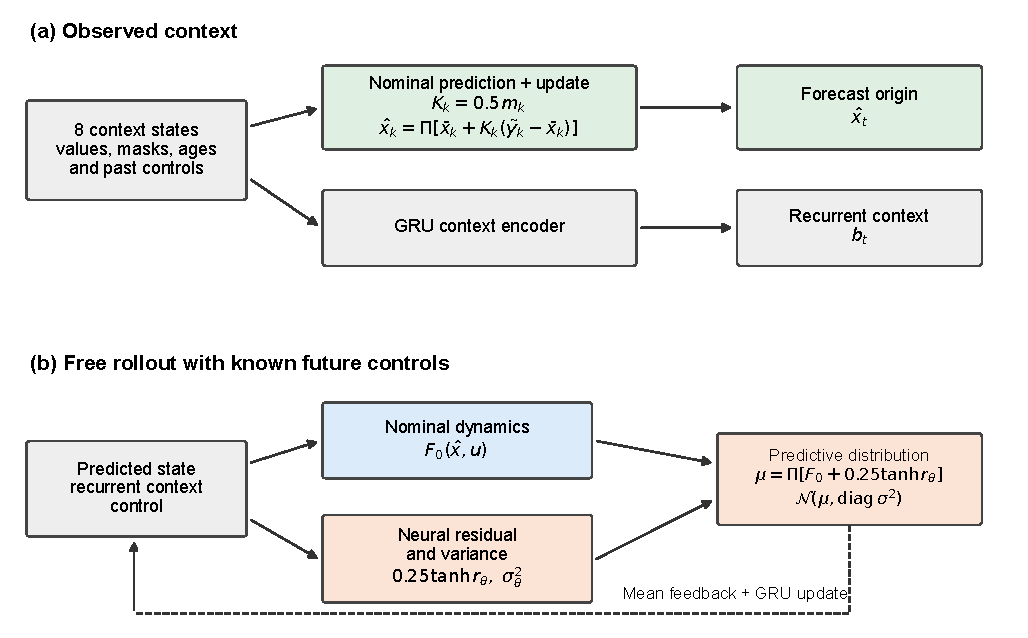
\includegraphics[width=0.92\textwidth]{figures/Fig1.pdf}
  \caption{Causal estimator--predictor interface. Nominal propagation and a
  mask-gated complementary update process the observed context. The corrected
  forecast origin initializes a nominal-plus-residual free rollout under a
  candidate future control sequence. No future observation is used during a
  rollout.}
  \label{fig:method}
\end{figure*}

\subsection{Problem formulation}

Let $\vect{x}_t\in\mathbb{R}^{d_x}$ be a physical state and
$\vect{u}_t\in\mathbb{R}^{d_u}$ a control. The available observation is
\begin{equation}
  \vect{y}_t=\vect{m}_t\odot(\vect{x}_t+\boldsymbol{\epsilon}_t),
\end{equation}
where $\vect{m}_t\in\{0,1\}^{d_x}$ is a channel mask. Missing entries are
filled by the latest available value, giving $\tilde{\vect y}_t$; the mask and
elapsed time since observation $\boldsymbol\delta_t$ remain model inputs.
Given an eight-step context and a candidate future control sequence, the model
predicts $H$ future states without teacher forcing.

\subsection{Mask-gated context update}

Let $F_0$ be a nominal dynamics step. Starting from the first imputed context
state, the filter alternates nominal prediction and measurement correction:
\begin{align}
 \bar{\vect x}_{k} &= F_0(\hat{\vect x}_{k-1},\vect u_{k-1}), \\
 \vect K_k &= \alpha\vect m_k,\qquad \alpha=0.5, \\
 \hat{\vect x}_k &= \Pi\!\left[\bar{\vect x}_k+
 \vect K_k\odot(\tilde{\vect y}_k-\bar{\vect x}_k)\right].
 \label{eq:filter}
\end{align}
An observed channel receives equal pre-projection weight from the nominal
prediction and measurement. A missing channel receives zero direct correction.
$\Pi$ is the identity except for the pendulum sine--cosine representation,
which is projected to the unit circle. The gain is fixed independently of
validation and test outcomes.

A gated recurrent unit (GRU) simultaneously encodes
$[\tilde{\vect y}_k,\vect m_k,\log(1+\boldsymbol\delta_k),\vect u_{k-1}]$.
Its final hidden state carries trajectory context into the rollout, but it does
not alter the measurement gain.

\subsection{Nominal-plus-residual rollout}

At future step $h$, the transition computes
\begin{align}
 \boldsymbol\mu^{p}_{t+h} &= F_0(\hat{\vect x}_{t+h-1},\vect u_{t+h-1}), \\
 [\vect r_{t+h},\vect \ell_{t+h}] &=
 R_\theta([\hat{\vect x}_{t+h-1},\vect u_{t+h-1},\vect b_{t+h-1}]), \\
 \boldsymbol\mu_{t+h} &= \Pi\!\left[
 \boldsymbol\mu^{p}_{t+h}+0.25\tanh(\vect r_{t+h})\right], \\
 \boldsymbol\sigma^2_{t+h} &=
 \max\{\exp(\operatorname{clip}(\vect\ell_{t+h},-8,4)),10^{-6}\}.
 \label{eq:rollout}
\end{align}
The residual is bounded to one quarter of a training standard deviation per
step in normalized coordinates. Predicted means feed the next transition, and
a GRUCell updates $\vect b$. The model minimizes mean diagonal Gaussian
negative log likelihood over all states and all 25 rollout steps:
\begin{equation}
 \mathcal L=\frac{1}{2Hd_x}\sum_{h=1}^{H}\sum_{q=1}^{d_x}
 \left[\log(2\pi\sigma_{hq}^2)+
 \frac{(x_{hq}-\mu_{hq})^2}{\sigma_{hq}^2}\right].
 \label{eq:nll}
\end{equation}

\subsection{Gain and error propagation}

For one observed scalar channel before a nonidentity projection, let
$e_p=\bar x-x$ be nominal prediction error and $\epsilon=y-x$ measurement
error. The filtered error is
$e_f=(1-\alpha)e_p+\alpha\epsilon$. With
$v_p=\mathbb E[e_p^2]$, $v_\epsilon=\mathbb E[\epsilon^2]$, and
$c=\mathbb E[e_p\epsilon]$,
\begin{equation}
 \mathbb E[e_f^2]=(1-\alpha)^2v_p+\alpha^2v_\epsilon
 +2\alpha(1-\alpha)c.
 \label{eq:mse}
\end{equation}
If $v_p+v_\epsilon-2c>0$, its constrained minimizer is
\begin{equation}
 \alpha^*=\operatorname{clip}_{[0,1]}
 \left(\frac{v_p-c}{v_p+v_\epsilon-2c}\right).
 \label{eq:alpha}
\end{equation}
Thus $\alpha=0.5$ is optimal only when $v_p=v_\epsilon$ and $c=0$. This
identity predicts regime dependence: cleaner measurements favor a larger gain,
whereas inaccurate nominal propagation favors stronger measurement correction.

If the rollout transition is locally $L$-Lipschitz with local error $\eta_h$,
\begin{equation}
 \|\hat{\vect x}_{t+H}-\vect x_{t+H}\|
 \le L^H\|\hat{\vect x}_t-\vect x_t\|
 +\sum_{h=0}^{H-1}L^{H-1-h}\eta_h.
 \label{eq:rollout_bound}
\end{equation}
The filter changes the initial-error term; the residual changes the accumulated
transition term. The component experiments estimate their separate effects.

\subsection{Receding-horizon use}

For each control step, the current eight-state context is processed once per
candidate sequence. Cross-entropy MPC samples bounded action sequences,
evaluates their predicted mean trajectories, retains the lowest-cost elites,
and applies the first action of the updated mean. The next optimization is warm
started by shifting that mean. The model is not retrained for the control
objective, and predictive variances are not used by this controller.


\section{Evaluation Design}

\subsection{Open-loop controlled benchmark}

The benchmark contains a damped oscillator, forced Duffing oscillator,
controlled Van der Pol oscillator, torque-driven pendulum, and cart--pole.
Fourth-order Runge--Kutta integration generates training, validation, and test
trajectories. Each of eight seeds independently draws the data and initializes
training. Methods share each seed--system data set.

Three test regimes are fixed: clean in-distribution (ID), corrupted ID, and
corrupted out-of-distribution (OOD) parameters. Corruption combines additive
measurement noise and channel missingness with causal carry-forward. Eleven
variants include recurrent, transformer, neural ODE, physics-guided, nominal,
and residual predictors plus filter-gain and training-horizon sensitivities.
Every learned method receives the same six-trial validation budget. The primary
metric is normalized root mean squared error at the 25-step horizon
(NRMSE-25), averaged equally across the 15 system--regime cells within each
seed.

The predeclared primary contrast compares \method{} with the PGNN-style model.
It requires a paired 95\% interval lower bound above a 5\% improvement and an
exact one-sided seed sign-flip $p<0.05$. The gated robustness claim additionally
requires improvement in the two corrupted regimes and noninferiority within
5\% on clean ID data. Component analyses compare the fixed filter plus nominal
rollout with the complete model, vary the residual multiplier at fixed weights,
and impose a synchronous two-step context outage.

\subsection{Frozen closed-loop regulation study}

The additional control study was specified before execution and reuses the
frozen PGNN-style and \method{} checkpoints. It includes all five systems,
eight seeds, and three plant/observation conditions: ID clean, ID corrupt, and
OOD-parameter corrupt. Four independently generated plant episodes populate
each seed--system--condition cell. Initial states, plant parameters,
observation draws, masks, and planner draws are paired across four prediction
interfaces: nominal propagation from the last imputed state, filter plus
nominal propagation, PGNN-style, and \method. ID clean and ID corrupt also
share the plant draw.

Seven zero-input transitions establish the eight-state context. The controller
then regulates for 20 steps. Deterministic-mean cross-entropy MPC uses horizon
8, 64 candidates, two iterations, and eight elites. Action sequences start
with standard deviation 0.6 of the action limit, with a 0.05 floor. The stage
objective is mean squared state error in training-standard-deviation units plus
0.01 times squared normalized action; terminal state error receives an
additional factor of two. The pendulum target is
$(\sin\theta,\cos\theta,\omega)=(0,1,0)$ and the other targets are zero.
Corrupt observations use Gaussian noise with scalar standard deviation 8\% of
the mean training-state standard deviation and 25\% independent channel
missingness.

The primary closed-loop response is the realized mean normalized state loss
over 20 controlled transitions. Episodes, systems, and conditions receive
equal weight within each seed. The reported \method{}--PGNN contrast is the
mean of eight seed-level relative improvements, with a 5,000-replicate paired
seed bootstrap interval and an exact one-sided sign-flip test against zero.
Controller settings were not changed after observing outcomes.

\subsection{Measured-flight external evaluation}

The NanoDrone experiment uses recorded states and motor commands from the
nonlinear system-identification benchmark \cite{busetto2026_nanodrone}. Three
held-out flights from a distinct trajectory family provide 387 forecast
windows. A reduced quadrotor prior omits parts of the recorded platform
dynamics; learned models have 47,000 parameters and use five training seeds.
The evaluation crosses four context conditions (recorded, added noise,
missingness, and both), two horizons (25 and 50), and four predictors
(\method, its unfiltered residual counterpart, a recurrent model, and the
nominal prior). It reports full-state NRMSE, position RMSE, velocity RMSE, and
marginal 95\% coverage. Flights receive equal weight before averaging training
seeds.

Training, test, and analysis artifacts are hash-checked before tables and
figures are generated. The supplementary material gives the system equations,
parameter ranges, tuning space, complete cell results, and artifact inventory.


\section{Results}

\subsection{Open-loop prediction}

Table~\ref{tab:open-loop} summarizes the cell-balanced confirmatory results.
At 25 steps, CFR-WM obtains NRMSE $\CFRNRMSE$ versus $\PGNNNRMSE$ for the
preselected PGNN-style comparator. The paired seed-level relative improvement
is \PrimaryImprovement\% (95\% fixed-cell bootstrap interval
[\PrimaryRelativeCILow\%, \PrimaryRelativeCIHigh\%]); the exact one-sided
sign-flip test against the 5\% practical margin gives
$p=\PrimaryPValue$. The corresponding absolute difference is
\PrimaryDifference{} (95\% interval [\PrimaryCILow,
\PrimaryCIHigh]). These quantities satisfy the predeclared aggregate
criterion.

\begin{table*}[!t]
  \caption{Open-loop prediction over five systems, three regimes, and eight
  paired seeds. Entries are mean $\pm$ SD across seed-level cell-balanced
  aggregates.}
  \label{tab:open-loop}
  \centering
  \footnotesize
  \begin{tabular}{lrrrr}
\toprule
Method & Mean parameters & NRMSE-1 & NRMSE-10 & NRMSE-25 \\
\midrule
CFR-WM & 57694 & 0.039 $\pm$ 0.001 & 0.057 $\pm$ 0.002 & \textbf{0.100 $\pm$ 0.004} \\
CFR-gain-0.25 & 57694 & 0.037 $\pm$ 0.001 & 0.059 $\pm$ 0.002 & 0.103 $\pm$ 0.004 \\
CFR-gain-0.75 & 57694 & 0.047 $\pm$ 0.001 & 0.065 $\pm$ 0.002 & 0.107 $\pm$ 0.005 \\
PGNN-style & 61275 & 0.060 $\pm$ 0.001 & 0.070 $\pm$ 0.002 & 0.110 $\pm$ 0.003 \\
CFR-gain-1 & 57694 & 0.059 $\pm$ 0.001 & 0.073 $\pm$ 0.002 & 0.114 $\pm$ 0.004 \\
PG-DMM-style & 61493 & 0.063 $\pm$ 0.001 & 0.075 $\pm$ 0.002 & 0.114 $\pm$ 0.003 \\
RSSM-style & 62485 & 0.073 $\pm$ 0.002 & 0.090 $\pm$ 0.005 & 0.123 $\pm$ 0.006 \\
Transformer-style & 59708 & 0.074 $\pm$ 0.002 & 0.094 $\pm$ 0.004 & 0.132 $\pm$ 0.009 \\
SimNorm-style & 62485 & 0.074 $\pm$ 0.002 & 0.098 $\pm$ 0.006 & 0.138 $\pm$ 0.013 \\
CFR-gain-0 & 57694 & 0.081 $\pm$ 0.003 & 0.100 $\pm$ 0.003 & 0.144 $\pm$ 0.005 \\
CFR-one-step & 57694 & 0.040 $\pm$ 0.001 & 0.136 $\pm$ 0.050 & 0.278 $\pm$ 0.104 \\
\bottomrule
\end{tabular}

\end{table*}

The regime split is asymmetric. Combining the corrupt-ID and corrupt-OOD
cells gives a \CorruptImprovement\% improvement (95\% interval
[\CorruptRelativeCILow\%, \CorruptRelativeCIHigh\%],
$p=\CorruptPValue$ against 5\%). On clean ID data the change is
\CleanImprovement\% (95\% interval [\CleanRelativeCILow\%,
\CleanRelativeCIHigh\%], $p=\CleanPValue$ against the $-5\%$
noninferiority margin). The clean component therefore does not satisfy the
predeclared gated robustness criterion. The system-level contrasts are also
heterogeneous: three clean-system cells deteriorate by more than 10\%, whereas
all five corrupt-ID cells favor CFR-WM.

\subsection{Component and outage analyses}

Table~\ref{tab:components} separates forecast-origin correction from residual
rollout. Filtering followed by nominal propagation reaches aggregate NRMSE
0.111, compared with 0.119 for CFR-WM and 0.132 for PGNN-style. Loading the
trained CFR-WM checkpoints and setting the inference residual multiplier to
zero reproduces the filter-plus-nominal result; increasing the multiplier from
0 to 0.5 increases mean error in every reported regime. Thus the learned
residual does not improve point accuracy in this experiment.

\begin{table*}[!t]
  \caption{Classical components and residual-scale sensitivity. The lower
  block changes only the inference-time residual scale of trained CFR-WM
  checkpoints.}
  \label{tab:components}
  \centering
  \footnotesize
  \begin{tabular}{lrrrr}
\toprule
Analysis and variant & All & Clean & ID corrupt & OOD corrupt \\
\midrule
Nominal, final imputation & 0.137 & 0.040 & 0.151 & 0.221 \\
Complementary filter + nominal & 0.111 & 0.042 & 0.092 & 0.201 \\
PGNN-style & 0.132 & 0.052 & 0.134 & 0.211 \\
CFR-WM & 0.119 & 0.055 & 0.097 & 0.204 \\
\midrule
CFR-WM, inference scale 0 & 0.111 & 0.042 & 0.092 & 0.201 \\
CFR-WM, inference scale 0.125 & 0.113 & 0.046 & 0.093 & 0.202 \\
CFR-WM, inference scale 0.25 & 0.119 & 0.055 & 0.097 & 0.204 \\
CFR-WM, inference scale 0.5 & 0.135 & 0.079 & 0.113 & 0.213 \\
\bottomrule
\end{tabular}

\end{table*}

A synchronous two-step all-channel context outage increases CFR-WM NRMSE by
2.7\%, from its matched clean reference, whereas PGNN-style increases by
51.9\%. This intervention isolates missing context observations; it does not
test longer outages or actuator faults.

\subsection{Receding-horizon regulation}

Table~\ref{tab:closed-loop} reports realized control outcomes over
\ClosedLoopEpisodes{} paired episodes. CFR-WM yields state loss
\ClosedLoopCFRLoss{} versus \ClosedLoopPGNNLoss{} for PGNN-style. The
seed-balanced relative improvement is \ClosedLoopImprovement\% (95\% paired
bootstrap interval [\ClosedLoopCILow\%, \ClosedLoopCIHigh\%]); the exact
one-sided sign-flip test against zero gives $p=\ClosedLoopPValue$. Mean
improvements favor CFR-WM in all 15 system--condition cells, ranging from
0.006\% for the damped-oscillator OOD-corrupt cell to 2.8\% for the
cart--pole corrupt-ID cell (Fig.~\ref{fig:closed-loop}).

\begin{table*}[!t]
  \caption{Closed-loop regulation with a common cross-entropy MPC controller.
  State loss and action effort are mean $\pm$ SD across eight seed-level
  aggregates. Condition columns report state loss.}
  \label{tab:closed-loop}
  \centering
  \footnotesize
  \begin{tabular}{lccccc}
\toprule
Controller & State loss & Action effort & ID clean & ID corrupt & OOD corrupt \\
\midrule
Nominal, last state & 0.372 $\pm$ 0.089 & 0.448 $\pm$ 0.013 & 0.362 $\pm$ 0.099 & 0.368 $\pm$ 0.098 & 0.385 $\pm$ 0.093 \\
Filter + nominal & 0.370 $\pm$ 0.090 & 0.398 $\pm$ 0.013 & 0.362 $\pm$ 0.099 & 0.364 $\pm$ 0.099 & 0.383 $\pm$ 0.092 \\
PGNN-style & 0.375 $\pm$ 0.091 & 0.464 $\pm$ 0.017 & 0.367 $\pm$ 0.100 & 0.370 $\pm$ 0.099 & 0.388 $\pm$ 0.094 \\
CFR-WM & 0.370 $\pm$ 0.090 & 0.404 $\pm$ 0.016 & 0.363 $\pm$ 0.099 & 0.364 $\pm$ 0.099 & 0.384 $\pm$ 0.092 \\
\bottomrule
\end{tabular}

\end{table*}

\begin{figure*}[!t]
  \centering
  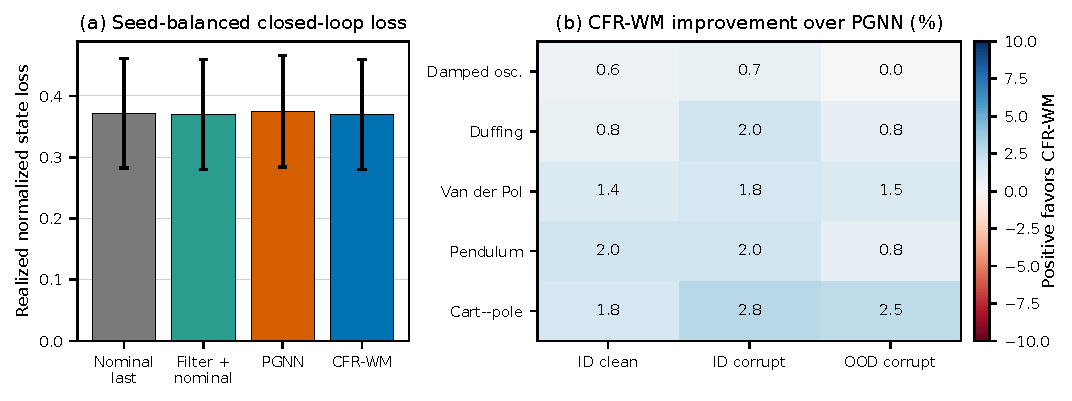
\includegraphics[width=0.92\textwidth]{figures/FigClosedLoop.pdf}
  \caption{Frozen closed-loop study. (a) Seed-balanced mean normalized state
  loss; error bars are one SD across eight seeds. (b) Mean CFR-WM improvement
  over PGNN-style within each system--condition cell. Positive values favor
  CFR-WM.}
  \label{fig:closed-loop}
\end{figure*}

The absolute separation between learned predictors is small. Filter plus
nominal dynamics obtains state loss \ClosedLoopFilterNominalLoss{}, slightly
below CFR-WM's \ClosedLoopCFRLoss{}, and also uses less action effort (0.398
versus 0.404). The nominal-last interface reaches \ClosedLoopNominalLoss{}.
Closed-loop performance therefore supports the value of context correction,
but not an additional benefit from the learned residual.

\subsection{Measured-flight transfer}

On held-out NanoDrone flights, CFR-WM improves 50-step position RMSE over the
matched unfiltered residual model in all four context conditions
(Table~\ref{tab:external-position}). For example, under combined noise and
missingness, position RMSE is $0.094\pm0.004$ m versus
$0.125\pm0.017$ m. The state components do not move uniformly: the unfiltered
model has lower 50-step full-state NRMSE in all eight context--horizon
comparisons, and it has lower velocity error for recorded and missing-only
contexts.

\begin{table*}[!t]
  \caption{External 50-step physical errors on three held-out NanoDrone
  flights. Entries are mean $\pm$ SD across five training seeds after equal
  weighting of flights.}
  \label{tab:external-position}
  \centering
  \footnotesize
  \begin{tabular}{lrrrr}
\toprule
& \multicolumn{2}{c}{Position RMSE (m)} & \multicolumn{2}{c}{Velocity RMSE (m/s)} \\
Context & CFR-WM & Unfiltered & CFR-WM & Unfiltered \\
\midrule
As recorded & $0.078 \pm 0.003$ & $0.083 \pm 0.010$ & $0.249 \pm 0.015$ & $0.233 \pm 0.009$ \\
Noise & $0.091 \pm 0.003$ & $0.115 \pm 0.007$ & $0.257 \pm 0.014$ & $0.258 \pm 0.007$ \\
Missing & $0.081 \pm 0.005$ & $0.095 \pm 0.022$ & $0.259 \pm 0.014$ & $0.243 \pm 0.009$ \\
Noise + missing & $0.094 \pm 0.004$ & $0.125 \pm 0.017$ & $0.267 \pm 0.014$ & $0.268 \pm 0.009$ \\
\bottomrule
\end{tabular}

\end{table*}

The probabilistic output is not calibrated for this transfer. CFR-WM's nominal
90\% marginal coverage ranges from 0.524 to 0.667 across the four context
conditions, compared with 0.565--0.779 for the matched unfiltered model. The
same CFR-WM intervals are narrower and have higher calibration error in every
condition. These intervals are therefore not used in the MPC objective.

\section{Discussion}

The experiments distinguish two mechanisms that are often combined inside a
single learned dynamics model. Complementary context correction reduces the
forecast-origin error in (\ref{eq:rollout_bound}); the learned residual is
intended to reduce accumulated transition error. Here the first mechanism is
consistently useful under observation corruption. It explains the
\CorruptImprovement\% open-loop gain, the outage response, and the reduction in
closed-loop action effort relative to PGNN-style. Its small closed-loop state
loss advantage is repeated across all system--condition means, although the
aggregate magnitude is only \ClosedLoopImprovement\%.

The residual evidence points in the other direction. Filter plus nominal
dynamics is better than the full model in both the post-hoc open-loop analysis
and the frozen closed-loop study. This result is compatible with a nominal
model that is accurate enough that the learned correction adds estimation
variance or compounds small one-step biases. Residual learning may still be
useful when mismatch is larger, but the current benchmark does not demonstrate
that benefit. A model-selection rule for automation should consequently retain
the zero-residual variant rather than assuming that an additional trainable
component improves control.

Equation~(\ref{eq:alpha}) also explains the clean-regime result. A fixed gain
of 0.5 assumes a particular relationship between nominal-prediction and
measurement errors. When measurements are clean, equal weighting can discard
useful measurement information; when measurements are corrupted, it can
suppress noise and bridge missing channels. A channel- and state-dependent
gain estimated without access to test outcomes is a direct extension. Its
evaluation should retain the same clean noninferiority gate because an
adaptive estimator can otherwise trade nominal accuracy for corruption
robustness.

The measured-flight study narrows the transfer claim. Position error improves,
whereas full-state error and interval coverage do not. The reduced quadrotor
prior omits platform effects, and the diagonal Gaussian head does not represent
cross-state or temporal dependence. Risk-sensitive control therefore requires
recalibration or a richer predictive distribution before using these
uncertainties as constraint margins.

The closed-loop experiment uses simulated plants, one deterministic-mean CEM
configuration, 20 control steps, and a quadratic regulation objective. The
measured flights provide real sensor and actuation records but not an online
intervention. Physical closed-loop experiments, task constraints, longer
missing-data bursts, informative sensor failures, and latency on the target
controller remain necessary to assess deployment performance. The bounded
residual and finite-horizon results do not by themselves establish closed-loop
stability.

\section{Conclusion}

CFR-WM separates a mask-gated complementary state update from a
nominal-plus-residual free rollout. Across a controlled open-loop benchmark,
the interface improves 25-step prediction under corrupted observations but
does not meet the clean-regime noninferiority criterion. In a frozen
receding-horizon study it reduces state loss relative to PGNN-style by
\ClosedLoopImprovement\%, while filter plus nominal dynamics remains slightly
better than the complete model. Measured flights show a position benefit
alongside worse full-state error and undercovered intervals. For the tested
automation setting, complementary context filtering is the supported design
element; residual and uncertainty components require stronger evidence before
they are used for control decisions.


\section*{Acknowledgment}
OpenAI ChatGPT/Codex was used for literature screening, language drafting and
editing, and assistance in drafting software and analysis scripts. The authors
verified the cited sources, equations, code, numerical results, and claims,
approved the manuscript, and take responsibility for its content.

\balance
\bibliographystyle{IEEEtran}
\bibliography{references}
\end{document}
